\documentclass[a4paper]{article}

\usepackage[utf8]{inputenc}
\usepackage[portuges]{babel}
\usepackage{a4wide}
\usepackage{graphicx}
\graphicspath{ {images/} }

\title{Projeto de Laboratórios de Informática 1\\Grupo 156}
\author{José Pedro Milhazes Carvalho Pinto A80741 \and Pedro Miguel Fernandes de Lima A80328}
\date{\today}

\begin{document}
\maketitle

\begin{abstract}
   Nesta unidade curricular, foi-nos proposta a implementação de uma versão nossa
   de um famoso jogo de vídeo de estratégia \textit{retro}, o \emph{"Bomberman"}.
   Este projeto foi executado utilizando a linguagem \emph{Haskell} e surge como o
   primeiro trabalho de programação neste curso de Engenharia Informática. Sendo esta
   uma linguagem de programação funcional, apresentou-se, sobretudo, como um desafio, 
   particularmente para novos estudantes de informática, no sentido em que exige um
   encadeamento perfeito entre raciocínios e o "encaixe" de diversas ferramentas, 
   mantendo um fluxo de informação na forma de \emph{input} e \emph{output} de funções,
   para construir cada tarefa.

    Ao longo da execução das tarefas envolvidas na construção
   e programação do jogo, servimo-nos de muitas ferramentas novas para nós, embora integrantes 
   do quotidiano da programação. Assim, este projeto foi uma introdução à programação,
   à maneira de pensar neste contexto, aos tipos de dados, ao teste e \textit{debug} do
   código, à utilização do sistemas de controlo de versões, à documentação de código, bem como
   de muitas outras práticas que farão de agora em diante parte do nosso trabalho.
\end{abstract}

\pagebreak







\tableofcontents









\pagebreak 

\section{Introdução}
\label{sec:intro}

  \hspace{0.54cm}A implementação do \textit{bomberman} foi dividida em duas fases, cada 
  uma com três tarefas.

  Na primeira, ficámos encarregues de apresentar soluções para a construção 
  do mapa inicial (sem os jogadores), para a reação a comandos, e para a 
  compressão de estados do jogo, sendo estas as tarefas 1, 2 e 3, respetivamente.

  Na segunda fase, a tarefa nº 4 correspondeu à reação à passagem do tempo,
  enquanto que a tarefa 5 concretizou a implementação do jogo, fazendo uso das 
  tarefas anteriores, e na tarefa 6 procedemos à programação de um bot que 
  jogasse \textit{bomberman}.

  Apesar de a tarefa 5 ser apenas refrida em 5º lugar (e na segunda fase), é
  importante reconhecer que toda a estrutura do trabalho e divisão de tarefas
  se deveu à logica de implementação do jogo seguida na tarefa 5, uma vez que
  esta faz uso da livraria \emph{Gloss} do \emph{Haskell}, utilizando o IO 
  \emph{play}, que utiliza, precisamente, um estado inicial (tarefa1), uma 
  função de reação ao tempo (tarefa 4), uma função de reação a comandos (tarefa
  2), uma função para desenhar na janela do programa um estado do jogo (própria 
  tarefa 5), se pretendido, uma função que controle certos jogadores (tarefa 6),
  entre outras especificações. 

  Neste relaório faremos uma breve descrição dos problemas a resolver e das
  ferramentas e estratégias que adotámos para implementar. Procederemos, então,
  a uma descrição mais detalhada de certos aspetos relativos às nossas soluções,
  e a uma reflexão conclusiva sobre todo o projeto e o seu resultado final.


\pagebreak










\section{Descrição do Problema}


Como já referido, o problema a resolver foi repartido:

\subsection{1ª Fase}





\subsubsection{Tarefa 1}

    \hspace{0.54cm}Comecámos este projeto por implementar uma função \texttt{mapa}, que, dada uma dimensão 
    e uma \textit{seed}, construisse um mapa inicial dessa dimensão e o preenchesse com elementos
    gerados a partir de uma lista pseudoaleatória gerada a partir da \textit{seed}.
    Esta primeira tarefa ajudou-nos a interiorizar o nosso objeto de estudo e de trabalho, pois
    o mapa, estando na forma de uma lista de \textit{Strings}, tinha de estar organizado de uma
    forma específica, obedecendo a certas regras, entre as quais:

    \begin{itemize}
      \item Os números da lista gerada apenas serão feitos corresponder a espaços que não sejam
            pedras fixas ou espaços vazios nos cantos.
      \item Os powerups gerados têm de estar organizados por ordenada e abcissa crescente, por esta 
            ordem.
      \item Independentemente das suas coordenadas, os powerups "flames" vêm sempre depois dos "bombs".
    \end{itemize}
    
    O resultado desta função podia ser imprimido no \texttt{stdout} e, sendo pseudoaleatório, testado
    ao ser comparado com uma soluçã correta.

\subsubsection{Tarefa 2}

    \hspace{0.54cm}Na segunda tarefa, era esperada a reação do jogo a comandos. O input desta função era o estado
    do jogo, o número de um dado jogador e a jogada que o mesmo pretendesse fazer. O output encontra-se
    no mesmo formato que o da tarefa 1, embora (representando este um jogo em curso) inclui jogadores
    e (possivelmente) bombas colocadas no mapa. Sendo a jogada posśivel, o estado é alterado, e,
    caso contrário, é devolvido o estado do jogo dado como input.

    Mais uma vez, esta tarefa é fácil de testar, procedendo-se da mesma forma que na tarefa anterior.

\subsubsection{Tarefa 3}
    \hspace{0.54cm}Nesta parte final da primeira fase, eram pedidas duas funções complementares, \texttt{encode} e 
    \texttt{decode}. Como o seu nome indica, estas funções codificam e descodificam, respetivamente,
    um dado estado do jogo. Esta codificação surge como um meio de armazenar um jogo em curso, tentando
    gastar o mínimo de informação (medida em número de carateres) possível. Esta rentabilização da 
    informação é feita, em síntese, eliminando informação reduntante.
    Estas funções recebiam um estado de jogo de produzem uma \texttt{string},e  vice-versa.

    Os testes a esta tarefa são feitos simplesmente verificando se a solução implementada de facto
    converte os estados em formatos menores sem perder (ou, pior, alterar) informação. 
    \begin{center}
    \texttt{decode \$ encode mapa = mapa}
    \end{center}

\pagebreak










\subsection{2ª Fase}

\subsubsection{Tarefa 4}
    \hspace{0.54cm}A tarefa 4 é parecida com a segunda, no sentido em que recebe um estado e gera um estado alterado
    por um acontecimento. Neste caso, o acontecimento que altera o estado do jogo é a passagem de cada 
    instante de tempo.
    Com a passagem do tempo, o timer das bombas é reduzido, as bombas cujo timer é 1 antes da passagem
    explodem, e, caso o instantes restantes até o jogo terminar sejam inferiores a $(d-2)^2$, sendo 
    $d$ a dimensão do mapa, fecha-se mais um espaço do mapa, segundo um padrão de espiral que começa
    no canto superior esquerdo.

    Esta tarefa é a última que pode ser testada da mesma forma que a 1 e a 2.


\subsubsection{Tarefa 5}
    \hspace{0.54cm}Na tarefa 5 surge a implementação propriamente dita do jogo. Embora estejam já implementadas
    soluções para reação a comandos e passagem do tempo, é necessário o desenvovimento de uma 
    interface gráfica, reproduzida a partir de um cada possível estado do jogo. O "esqueleto"
    do \texttt{IO play} já se encontrava definido. Coube-nos importar as tarefas anteriores e 
    reproduzir graficamente o jogo. Compilada esta tarefa, deve resultar o produto final deste projeto,
    o jogo propriamente dito. 


\subsubsection{Tarefa 6}
    \hspace{0.54cm}Por último, foi apresentado o desafio de desenvolver um bot que jogasse \textit{Bomberman}, 
    implementando uma função que, recebendo um estado do jogo e o tempo do mesmo, devolve a
    jogada (ou \texttt{Nothing}, no caso de o joador nao querer efetuar nenhum movimento).
    Qualquer implementação do bot que tivesse um \textit{output} inválido seria eliminada do jogo, 
    na avaliação automática.
    





\pagebreak













\section{Concepção da Solução}

    \hspace{0.54cm}Segue-se uma descrição das estratégias que adotámos para desenvolver as soluções 
    para os problemas apresentados.

\subsection{Estruturas de Dados}

    \hspace{0.54cm}As estruturas de dados de maior destaque, neste trabalho foram as que se apresentam 
    na lista seguinte. Consistem maioritariamente em \textit{types}definidos por mera comodidade sintática e de legibilidade do código. \hspace{12 cm}


    \begin{itemize}
    \item  \texttt{type Mapa   = [String]}
              \linebreak
              \raggedright{Tipo que representa o estado do jogo numa lista de strings}
              \linebreak
    \item  \texttt{type Estado = ([String],[Brick],[Brick],[Powerup],[Bomb],[Player],Float, String)}
              \linebreak 
              \raggedright{"Cápsula" de informação extraída do tipo \texttt{Mapa}, adaptada à sua
                          utilidade na tarefa 5, e informação relativa ao estado do programa do jogo}
              \linebreak
    \item  \texttt{type State  = ( Mapa, [Cords], [Cords], [Powers], [Bombs] , [Players])}
              \linebreak
              \raggedright{"Cápsula" de informação extraída do tipo \texttt{Mapa}, adaptada
                           à sua utilidade na tarefa 6}
              \linebreak
    \item  \texttt{type Cords  = (Int,Int)}
              \linebreak 
              \raggedright{Par de números inteiros que representam coordenadas no mapa do jogo.}
              \linebreak
    \item  \texttt{data RPath a = C a [RPath a] deriving (Eq, Show)}
              \linebreak 
              \raggedright{Estrutura que nos permitiu representar uma árvore de caminhos possíveis a 
                           partir de nodos numa rede, na tarefa 6}
    \end{itemize}
    
    Nas últimas tarefas, o tipo \texttt{Mapa} serviu simplesmente como \textit{input}, tendo nós
    convertido o mesmo para outras estruturas de dados mais apropriadas para trabalhar.
    Há que notar que o mesmo elemento (i.e. bombas, powerups, jogadores), foi encarado 
    de formas diferentes em tarefas diferentes, tendo em conta a informação relevante
    para a solução do problema em questão. Por exemplo, na tarefa 5 retirámos
    toda a informação relativa a cada bomba, enquanto que na tarefa 6 apenas aproveitámos
    o \textit{timer} de cada bomba e os espaços que seriam afetados pela sua explosão.
\pagebreak












\subsection{Implementação}

    \hspace{0.54cm}Segue-se uma \textit{overview} da nossa solução para as diferentes tarefas. Por uma questão
    de simplicidade, os exemplos apresentados referem-se sempre ao mapa de dimensão 9 e \textit{seed} 0,
    ou alterações do mesmo.
    \subsubsection{Tarefa 1}
       \hspace{0.54cm} Na tarefa 1, nossa estratégia passou por, primeiro, gerar o esqueleto do mapa de dimensão $d$ 
        preenchido com o caracter 'X' nos espaços vazios dos cantos. \hspace{5cm}
        \linebreak
        \texttt{
        \linebreak \#\#\#\#\#\#\#\#\#
        \linebreak \#XX\ \ \ XX\#
        \linebreak \#X\# \# \#X\#
        \linebreak \#\ \ \ \ \ \ \ \#
        \linebreak \# \# \# \# \#
        \linebreak \#\ \ \ \ \ \ \ \#
        \linebreak \#X\# \# \#X\#
        \linebreak \#XX\ \ \ XX\#
        \linebreak \#\#\#\#\#\#\#\#\#}
        \linebreak

    Seguidamente, substituimos os espaços vazios pelos caracteres correspondentes aos números da lista
    gerada pseudoaleatoriamente. Os 'X' são substituídos por espaços vazios.\hspace{10cm}
        \linebreak
        \texttt{
        \linebreak \#\#\#\#\#\#\#\#\#
        \linebreak \# \ \  \ \ \ \ \#
        \linebreak \# \#?\#+\# \#
        \linebreak \#\ \ +\ \ ?\ \#
        \linebreak \#?\# \# \#?\#
        \linebreak \#\ \ \ \ !\ \ \#
        \linebreak \#X\#?\#?\# \#
        \linebreak \# \ ??\ \ \ \#
        \linebreak \#\#\#\#\#\#\#\#\#}
        \linebreak
    
     É aplicada uma função que substitui os caracteres \texttt{'!'} e \texttt{'+'} por \texttt{'?'} e regista a informação desses powerups em linhas que seguem o mapa propriamente dito.\hspace{10cm}
        \linebreak
        
        \texttt{>mapM\_ putStrLn \$ mapa 9 0
        \linebreak \#\#\#\#\#\#\#\#\#
        \linebreak \# \ \  \ \ \ \ \#
        \linebreak \# \#?\#?\# \#
        \linebreak \#\ \ ?\ \ ?\ \#
        \linebreak \#?\# \# \#?\#
        \linebreak \#\ \ \ \ ?\ \ \#
        \linebreak \#X\#?\#?\# \#
        \linebreak \# \ ??\ \ \ \#
        \linebreak \#\#\#\#\#\#\#\#\#
        \linebreak + 5 2
        \linebreak + 3 3
        \linebreak !\hspace{0.20cm}5 5}
        
        
\pagebreak

\subsubsection{Tarefa 2}
\hspace{0.54cm}Na segunda tarefa, dado o input do jogador e do caracter representativo da jogada, é primeiro testado 
    se a jogada é possível, e, em caso afirmativo, o mapa é reescrito com o jogador na sua nova posição, 
    eventuais powerups adicionados à sua \textit{string} e 
    a lista de powerups atualizada (caso tenha mudado), ou a bomba colocada nas coordenadas do jogador.
    \hspace{10cm}
    \linebreak
    
\texttt{>mapM\_ putStrLn  mapa
        \linebreak \#\#\#\#\#\#\#\#\#
        \linebreak \# \ \  \ \ \ \ \#
        \linebreak \# \#?\#?\# \#
        \linebreak \#\ \ ?\ \ ?\ \#
        \linebreak \#?\# \# \#?\#
        \linebreak \#\ \ \ \ ?\ \ \#
        \linebreak \#X\#?\#?\# \#
        \linebreak \# \ ??\ \ \ \#
        \linebreak \#\#\#\#\#\#\#\#\#
        \linebreak + 3 3
        \linebreak + 5 5
        \linebreak * 7 7 1 1 10
        \linebreak 0 4 3 +
        \linebreak 1 7 7 
        \linebreak 
        \linebreak
        >mapM\_ putStrLn \$ move mapa 0 'L'
        \linebreak \#\#\#\#\#\#\#\#\#
        \linebreak \# \ \  \ \ \ \ \#
        \linebreak \# \#?\#?\# \#
        \linebreak \#\ \ ?\ \ ?\ \#
        \linebreak \#?\# \# \#?\#
        \linebreak \#\ \ \ \ ?\ \ \#
        \linebreak \#X\#?\#?\# \#
        \linebreak \# \ ??\ \ \ \#
        \linebreak \#\#\#\#\#\#\#\#\#
        \linebreak + 5 5
        \linebreak * 7 7 1 1 10
        \linebreak 0 3 3 ++
        \linebreak 1 7 7 
        \linebreak  }    
    
\pagebreak

\subsubsection{Tarefa 3}
    \hspace{0.54cm}Quanto ao problema de compressão e descompressão, o tratamento que fizemos ao \texttt{Mapa} foi,
    nesta ordem:
    \begin{itemize}
    \item Inserção dos powerups das linhas abaixo no mapa propriamente dito (com caracteres diferentes
          para distinguir os tapados dos destapados)
    \item Remoção dos cardinais e dos espaços vazios fixos dos cantos.
    \item Codificação dos espaços vazios seguidos em números e tijolos ('?') seguidos em letras
    \item Mapeamento de padrões de conjuntos de 2 caracteres em 1 caracter maiúsculo
    \item Repetição do passo anterior, mas mapeando letras e números para outros símbolos, como parêntesis,
          por exemplo 
    \end{itemize}
    
    \texttt{>encode \$ mapa 9 0 \linebreak
               \hspace{3cm}"9.8a+3+\%""\%2!II"} \linebreak

    A função \texttt{decode} utiliza funções complementares na função inversa, como seria de esperar.\linebreak

    \texttt{>mapM\_ putStrLn \$ decode "9.8a+3+\%""\%2!II"
        \linebreak \#\#\#\#\#\#\#\#\#
        \linebreak \# \ \  \ \ \ \ \#
        \linebreak \# \#?\#?\# \#
        \linebreak \#\ \ ?\ \ ?\ \#
        \linebreak \#?\# \# \#?\#
        \linebreak \#\ \ \ \ ?\ \ \#
        \linebreak \#X\#?\#?\# \#
        \linebreak \# \ ??\ \ \ \#
        \linebreak \#\#\#\#\#\#\#\#\#
        \linebreak + 5 2
        \linebreak + 3 3
        \linebreak !\hspace{0.20cm}5 5}
    
\pagebreak

\subsubsection{Tarefa 4}

\hspace{0.54cm}Nesta tarefa começamos por reduzir o \textit{timer} das bombas todas do mapa em 1, e devolver esse mapa 
    como \textit{input} para uma função que faz explodir as bombas cujo timr esteja em 0.
    Desenvolvemos 4 funções recursivas semelhantes para calcular o efeito da explosão de uma bomba nas 4 direções,
    sendo o \textit{range} da bomba um argumento que decresce a cada espaço que as chamas percorrem. Os casos de 
    paragem são os tijolos, as pedras fixas, os \textit{powerups} ou um \textit{range} de 0. 
    
    Inicialmente, pensámos em simplesmente dar o \textit{output} da função que trata da explosão de uma bomba como
    \textit{input} para as chamadas da mesma função ao rebentar bombas que explodissem no mesmo instante, no entanto,
    apercebemo-nos de que isso criaria situações como, por exemplo, bombas explodirem simultaneamente e partirem 
    dois tijolos, ou irem para além de um \textit{powerup}.  
    
    Assim, criámos uma função que juntava mapas resultantes dessas explosões isoladas, e depois
    implementámos uma forma de fundir os elementos dessa mesma lista, de maneira que os tijolos que não constem
    em todos os mapas deixam de existir, bem como powerups, jogadores, e bombas. As bombas que, com as mesmas
    coordenadas, prevalecem são as que têm o \textit{timer} em 1, por terem sido afetadas por uma explosão.
    \hspace{6.5cm} \linebreak

    
    Caso o tempo seja inferior a $(d-2)^2$, o processo é o mesmo, mas é aplicada ao resultado uma função que,
    depois de calcular uma lista ordenada das coordenadas a ser esmagadas pela espiral, coloca um cardinal na 
    posição do mapa que seja igual ao elemento dessa mesma lista, de índice $(d-2)^2 -t$, sendo $t$ o argumento
    relativo ao tempo da função \texttt{avanca}. Qualquer string que tenha informação relativa a essas coordenadas
    é eliminada. \hspace{3cm}
    \linebreak
    
    \texttt{>mapM\_ putStrLn  mapa
        \linebreak \#\#\#\#\#\#\#\#\#
        \linebreak \#\#\ \  \ \ \ \ \#
        \linebreak \# \#?\#?\# \#
        \linebreak \#\ \ ?\ \ ?\ \#
        \linebreak \#?\# \# \#?\#
        \linebreak \#\ \ \ \ ?\ \ \#
        \linebreak \#X\#?\#?\# \#
        \linebreak \# \ ??\ \ \ \#
        \linebreak \#\#\#\#\#\#\#\#\#
        \linebreak + 3 3
        \linebreak + 5 5
        \linebreak * 7 7 1 1 1
        \linebreak 0 4 3 +
        \linebreak 1 7 7 
        \linebreak 
        \linebreak
        >mapM\_ putStrLn \$ avanca mapa 48
        \linebreak \#\#\#\#\#\#\#\#\#
        \linebreak \#\#\#\  \ \ \ \ \#
        \linebreak \# \#?\#?\# \#
        \linebreak \#\ \ ?\ \ ?\ \#
        \linebreak \#?\# \# \#?\#
        \linebreak \#\ \ \ \ ?\ \ \#
        \linebreak \#X\#?\#?\# \#
        \linebreak \# \ ??\ \ \ \#
        \linebreak \#\#\#\#\#\#\#\#\#
        \linebreak + 3 3
        \linebreak + 5 5
        \linebreak 0 4 3 + } 
    
\pagebreak

\subsubsection{Tarefa 5}
\hspace{0.54cm}Na implementação do jogo, recorrendo ao \emph{Gloss}, grande parte do trabalho já estava feita, tendo em conta 
    que as outras tarefas funcionam como "peças" para o funcionamento do mesmo. 
    
    No que toca à componente gráfica, procedemos à recolha de imagens dentro do mesmo tema e, recorrendo a um editor
    de imagem procedemos ao devido tratamento, de forma a o ambiente visual ser coerente (i.e. mesmas cores de fundo). Alguns exemplos: \hspace{4.5cm}
    \linebreak
    \begin{center}
    \texttt{
    
\includegraphics[scale=0.5]{powerup_bombs.jpg} 
\includegraphics[scale=0.5]{0.jpg}
    
\includegraphics[scale=0.5]{powerup_flames.jpg}\hspace{0.15cm}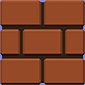
\includegraphics[scale=1.87]{brick.jpg}
    
\includegraphics[scale=0.38]{rocks.jpg}         
\includegraphics[scale=0.5]{bomb1.jpg}} \end{center}

    
    Criámos um \textit{type} \texttt{Estado} para encapsular a informação que pretendemos, sobretudo com listas de túpulos
    representativos dos diferentes objetos do jogo e as suas coordenadas, para facilmente associar essas listas a imagens
    e devolver uma lista de imagens desses objetos. Para tal efeito implementámos uma unção \texttt{placeMe} que, dado
    um par de coordenadas, a dimensão do mapa e uma imagem, redimensiona e coloca corretamente no mapa essa imagem. 

    
    Um dos componentes do tipo \texttt{Estado} é uma string indicativa do "ecrã"  em que o jogo se encontra, de modo a 
    permitir que haja diversas "fases" do programa, com o objetivo de criar menus de escolha da dimensão do mapa e do
    número de jogadores. \hspace{4cm}
    \linebreak
    
    Em vez de importar a tarefa 4 para gerir a passagem do tempo, criámos um módulo semelhante, mas com uma alternativa
    à função \texttt{avanca} que, para além do \texttt{Mapa} alterado, devolve também (num túpulo) uma lista com as 
    coordenadas que irão ter chamas na representação gráfica (e o tipo de chama em cada espaço). Na função reação ao
    tempo chamámos a função \texttt{bot} da tarefa 6 para controlar os bots, caso haja 3 ou mais jogadores.
   
    
    A reação a eventos conta com o controlo de dois jogadores, com as teclas de direções e as W, A, S, e D, bem
    como, para colocar bombas, das teclas C e M.  Quando há mais de 3 ou 4 jogadores, estes são controlados pelo bot
    implementado na tarefa 6.\hspace{3cm}
\linebreak

\begin{center}
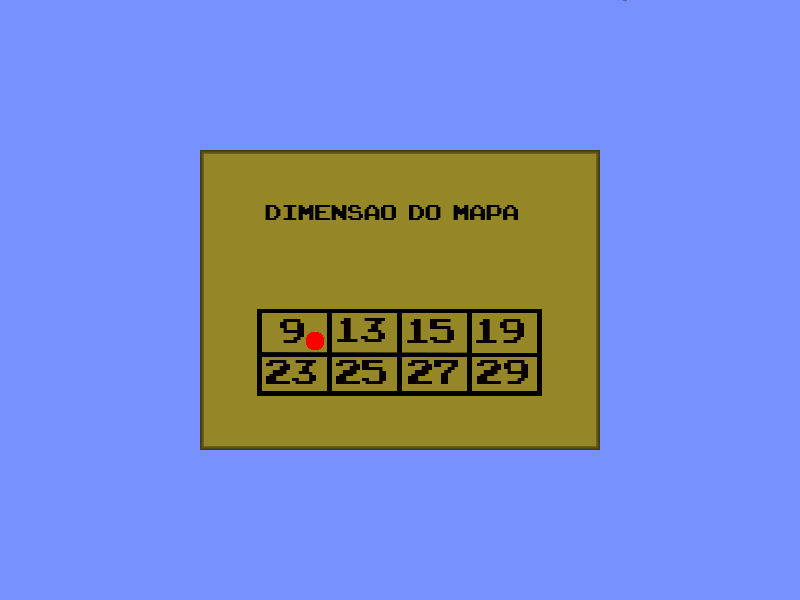
\includegraphics[scale=0.20]{dim.jpg}  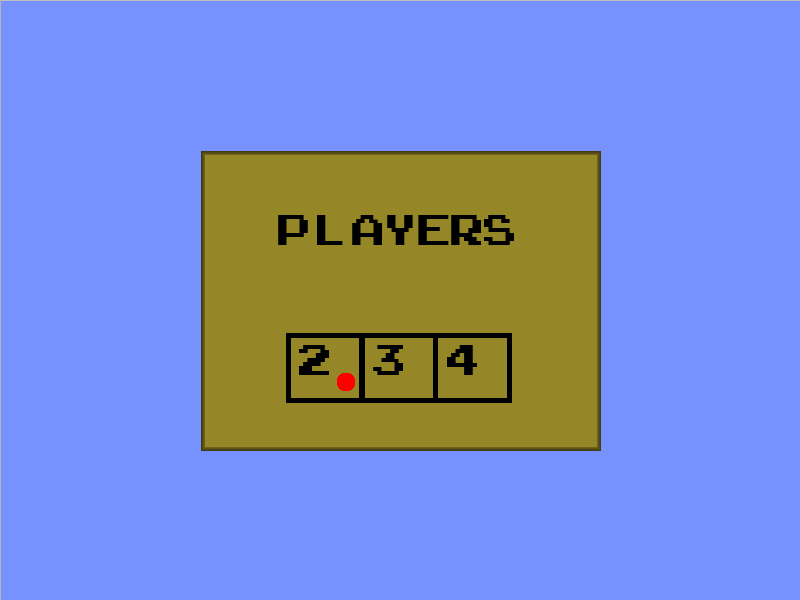
\includegraphics[scale=0.20]{players.jpg}
\end{center}

\begin{center}
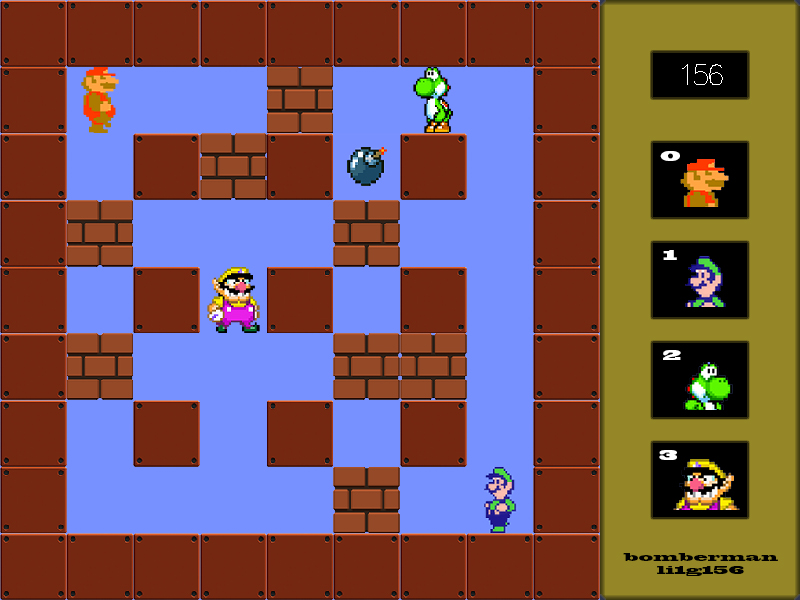
\includegraphics[scale=0.20]{game.jpg} 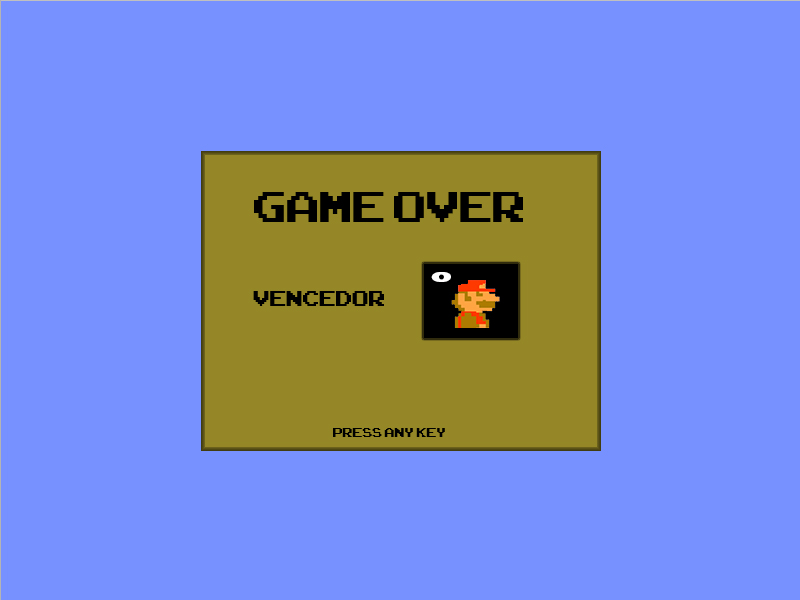
\includegraphics[scale=0.20]{over.jpg} 
\end{center}

\pagebreak

\subsubsection{Tarefa 6}
\hspace{0.54cm}A tarefa 6 foi a mais complexa. Começámos por implementar ferramentas básicas que nos ajudaram a perceber, 
    progressivamente, como programar o bot. Tal como fizemos anteriormente definimos um tipo \texttt{State} adequado
    ao problema. Ao ter incluído neste túpulo uma lista com as coordenadas de todos os lugares vazios no mapa,
    percebemos que podíamos aproveitar isto para desenvolver um sistema de locomoção, tendo em conta que o bot apenas 
    se move por espaços vazios.
    \linebreak
    
    Criámos uma função que, dado um estado e um par de coordenadas (a posição do bot), obtem a lista de todos os espaços vazios do mapa que estão ligados a esse mesmo espaço, direta ou indiretamente por espaços vazios, ao obter os espaços vazios adjacentes às coordenadas iniciais, e repetir o processo para esses mesmos espaços obtidos. 
    Assim criámos uma rede em que cada nodo é um espaço vazio ligado às coordenadas do jogador.
    
    Tomemos este mapa como exemplo para toda esta tarefa: \hspace{6cm}  
    \linebreak
    
    \texttt{>mapM\_ putStrLn  mapa
        \linebreak \#\#\#\#\#\#\#\#\#
        \linebreak \# \ \  \ \ \ \ \#
        \linebreak \# \#?\#\ \# \#
        \linebreak \#\ \ \ \ \ ?\ \#
        \linebreak \#?\# \# \#?\#
        \linebreak \#\ \ \ \ ?\ \ \#
        \linebreak \#X\#?\#?\# \#
        \linebreak \# \ ??\ \ \ \#
        \linebreak \#\#\#\#\#\#\#\#\#
        \linebreak + 3 3
        \linebreak + 5 5
        \linebreak * 7 7 1 1 10
        \linebreak 0 4 3 +
        \linebreak 1 7 7 
        \linebreak 
        \linebreak
        >let (a,b,c,d,e,f) = mkState mapa \linebreak
        >let s = (a,b,c,d,e,f)            \break
        >nub \$ network 10 b (4,3)        \break
        [(7,3),(7,2),(7,1),(1,2),(1,1),(2,1),(3,1),(4,1),(6,1),(5,1),(5,2),(5,4),\break
        (5,3),(4,5),(3,5),(1,3),(2,3),(3,4),(4,3),(3,3)]
         }
    \linebreak
    
    Utilizando essa rede, implementámos uma forma de encontrar um caminho entre dois nodos dessa rede, utilizando 
    \textit{rose trees}, ou \textit{multi-way trees} que representam os caminhos possíveis. Sabendo o destino
    pretendido, retiramos dessa árvore os caminhos que passam (e terminam, tendo em conta que definimos a ocorrência
    dessas coordenadas como um ponto de paragem na recursividade) pelo destino, e escolhemos o caminho com menos passos
    (ou ramos na árvore). Infelizmente tivemos de limitar o numero de passos para determinar redes, uma vez que, a partir
    de um certo número de nodos, os cálculos ficavam excessivamente grandes para ser resolvidos em tempo útil.
    \linebreak
    
    \texttt{>mkPathTree 10 (4,3) (1,1) (nub \$ network 10 b (4,3) \break
    C (4,3) [C (5,3) [C (5,2) [C (5,1) [C (4,1) [C (3,1) [C (2,1) [C (1,1) []]]],\break
    C (6,1) [C (7,1) [C (7,2) [C (7,3) []]]]]],C (5,4) []],C (3,3) [C (2,3) [C (1,3)\break
     [C (1,2) [C (1,1) []]]],C (3,4) [C (3,5) [C (4,5) []]]]]
    }
    \linebreak
    
    Criámos também uma função para descobrir uma alternativa a um destino, caso este não conste na rede de espaços vazios 
    ligados ao bot, baseada na distância de cada um dos nodos dessa mesma rede ao destino inicial, onde o bot larga uma
    bomba por estar no sítio mais próximo ao destino e não conseguir progredir, expandindo assim a rede e aproximando-se
    do espaço pretendido. Estando implementado o sistema de locomoção do bot, precisamos apenas da sua posição e de um destino, para lhe dar ordens. \hspace{13cm}
    \linebreak
    
    \texttt{>findWay 10 s (4,3) (1,1) \break
    "LLLUU"
    }
    \linebreak
    
    A definição do destino é o que varia tendo em conta o estado do jogo. No tipo \texttt{State} que criámos também
    está incluída uma lista de coordenadas que serão afetadas por futuras explosões. Assim, programámos o bot para
    ir para o sítio mais próximo que não estivesse em risco.\hspace{12cm}
        \linebreak
    
    \texttt{>runAway 10 s (7,7) \break
    "LL"
    }
    \linebreak
    
    
    Sendo o primeiro objetivo do bot fugir dos locais de morte iminente, o segundo é dirigir-se para o centro do mapa. 
    A estratégia que implementámos é, sobretudo, defensiva. Chegando ao centro do mapa, o bot espera pacientemente pelo
    final do jogo, fugindo às bombas dos seus inimigos e da espiral que vai fechando o mapa. Programámo-lo, no entanto, 
    para quando faltem 10 instantes para a partida acabar, colocar uma bomba e não tentar fugir dela, na expectativa 
    de que os outros bots o façam e sejam consumidos pela espiral. No caso de o bot se encontrar no centro do mapa aos 
    10 instantes para o fim do jogo, é impossível que não empate ou ganhe a partida.

    
    

\pagebreak

\subsection{Testes}

\hspace{0.54cm}Os testes desempenharam um papel importante ao longo deste projeto, tendo em conta que nos permitiram detetar
    muitos erros de raciocínio. Para as tarefas 1, 2, 3 e 4, fizemos uso dos testes que produzimos, compilando as tarefas
    e avaliando se cada resultado era o esperado. Por exemplo:
    \linebreak
    
    \texttt{>for((i=1;i<=20;i++)) do ./Tarefa4 999 <\textasciitilde/li1g156/tests/exemplo\$i.txt ; done}
    \linebreak
    
    A implementação do jogo no \emph{Gloss} ajudou-nos tambem a detetar um erro na tarefa 2 que nos tinha escapado
    na primeira fase, e permitiu-nos testar o bot. \hspace{4.5cm}
    \linebreak
    
\pagebreak












\section{Conclusões}

\hspace{0.54cm}Em conclusão, consideramos que este projeto contribuiu fortemente para a nossa aquisição de bons hábitos de trabalho, desde
    estratégias de \textit{debug}, estruturação de código, uso de \textit{data types}, documentação, controlo de versões
    e utilização de repositórios, e construção de testes. A aprendizagem mais relevante, para nós, foi a importância
    da planificação e desenvolvimento de ferramentas elementares antes de iniciar a implementação de uma solução para
    um problema minimamente complexo.
    
	
	    Na nossa opinião, o uso exclusivo do \emph{Haskell} não facilita o desenvolvimento de jogos, 
    uma vez que muitos aspetos e características do jogo têm de ser constantemente calculados,
    mesmo sem terem mudado. Sendo possível simplesmente armazenar certas variáveis e ir mudando
    os seus valores ao longo do decurso de um programa, a maior parte dos problemas ficariam
    mais fáceis de resolver, com poucos ou mesmo sem compromissos em termos de utilização de
    recursos do sistema.
    
    
    Quanto aos objetivos do trabalho, foram, de forma geral, cumpridos. Todas as tarefas funcionam como esperado e 
    desenvolvemos, nas tarefas de resposta mais abertas, soluções com um bom nível de desempenho recorrendo aos conhecimentos
    de que dispúnhamos.


\end{document}\grid
\grid\grid
\grid
